\chapter{The Hiring Filter: Skills, Traits, and Early Team Judgment}

This chapter follows a short School of Hard Knocks entrepreneurship interview segment, curated by LazyingArt LLC through Video2Book. The question is direct: when we are building a company or launching a venture, what makes someone worth bringing onto the team? The answer unfolds in a disciplined order. First we notice natural role fit. Then we ask whether role fit and visible talent are enough. Finally we arrive at the speaker's non-negotiable filter: coachability, humility, and persistence.

\section{The Founder’s Selection Problem}

The opening is not a general theory of personality. It is a founder's selection problem. We are trying to decide who belongs inside a young company, where each new person changes the working character of the whole firm.

Let \(c\) denote a candidate. The first thing the speaker allows us to notice is the candidate's apparent lane:
\begin{equation}
  c \longmapsto \operatorname{RoleType}(c).
\end{equation}
In the transcript, the examples are concrete:
\begin{equation}
  \operatorname{RoleType}(c)
  \in
  \{\text{sales},\ \text{engineering},\ \text{operations},\ldots\}.
\end{equation}
These are not scientific categories. They are practical founder labels. A sales type may naturally persuade and close. An engineering type may naturally build. An operations type may naturally impose order on repeated work.

The important point is that the speaker does not dismiss aptitude. He begins by granting it. People do have things they are good at, and a founder has to see those things. But the lecture immediately prepares the pivot: knowing what a person is good at is not the same as knowing whether that person should be on the team.

\section{Role Fit Is a Signal, Not a Decision}

A candidate's role type tells us where contribution might happen. It does not yet tell us whether the person can be built with, corrected, redirected, or trusted through difficulty.

We may write the useful direction as:
\begin{equation}
  \operatorname{Hire}(c)
  \Rightarrow
  \operatorname{RoleFit}(c)
  \quad\text{is a reasonable founder expectation.}
\end{equation}
If we bring someone into an early team, there should be some role in which that person can plausibly create value. But the reverse direction is the dangerous one:
\begin{equation}
  \operatorname{RoleFit}(c)
  \nRightarrow
  \operatorname{Hire}(c).
\end{equation}
That failed implication is the hinge of the passage. The speaker is not saying that talent is irrelevant. He is saying that talent is incomplete evidence.

\subsection{Question \& Answer}

\paragraph{Question.}
If someone is visibly talented, or clearly belongs to a useful role type, is that enough reason to bring the person onto the team?

\paragraph{Answer.}
No. The answer turns on the distinction between what can be taught and what must already be present. The speaker's practical claim is:
\begin{equation}
  \text{skills can be taught}
  \qquad\text{but}\qquad
  \text{traits cannot be reliably taught.}
\end{equation}
This should be read as a hiring judgment, not as a universal theorem about human beings. Inside this interview, it means that a founder may be able to train a person into a role, but cannot safely assume that humility, coachability, and persistence will appear after the offer letter is signed.

\section{Skill Updates and Trait Constraints}

To make the logic explicit, let \(S_t(c)\) represent the candidate's skill at time \(t\). If a person can learn, then training, practice, and feedback may increase skill:
\begin{equation}
  S_{t+1}(c)
  =
  S_t(c)+\Delta S_t(c),
  \qquad
  \Delta S_t(c)>0.
\end{equation}
This is the teachable part of the system. The company can improve a sales script, a technical process, an operational routine, or a management habit.

But that update rule hides a condition. The person must be able to receive correction. If coachability and humility are absent, the update is blocked. We can express the condition schematically as:
\begin{equation}
  \Delta S_t(c)>0
  \quad\text{requires}\quad
  \operatorname{Coachable}(c)
  \land
  \operatorname{Humble}(c).
\end{equation}
Persistence matters when the update is slow or uncomfortable:
\begin{equation}
  \operatorname{LearningThroughDifficulty}(c)
  \Rightarrow
  \operatorname{Persistent}(c).
\end{equation}
The notation is only a compact reconstruction of the spoken idea. The underlying mechanism is simple: skill improves only when the person can be taught, corrected, and kept in motion long enough for the improvement to matter.

\section{The Non-Negotiable Trait Set}

After the teachable-skill distinction, the speaker names the non-negotiables. He explicitly demotes the signals that often dominate hiring conversations: talent, school, referrals, and prior company prestige. Those may be positive signs, but they do not settle the decision.

The stated trait set is:
\begin{equation}
  \mathcal{T}
  =
  \{\text{coachable},\ \text{humble},\ \text{persistent}\}.
\end{equation}
A candidate clears the trait screen only when all three are present:
\begin{equation}
  \operatorname{TraitClear}(c)
  =
  \operatorname{Coachable}(c)
  \land
  \operatorname{Humble}(c)
  \land
  \operatorname{Persistent}(c).
\end{equation}
This is the speaker's practical non-negotiable filter. It does not claim that these are the only virtues in business. It says that, for this hiring decision, talent is not enough unless these traits make the talent usable.

\begin{table}
\centering
\begin{tabular}{|p{0.25\linewidth}|p{0.31\linewidth}|p{0.30\linewidth}|}
\hline
Signal & What it may show & What it does not prove \\
\hline
Sales, engineering, or operations type & A natural lane for contribution & That the person can learn inside this firm \\
\hline
Talent & Existing ability or performance & That the person is coachable or humble \\
\hline
School or referral & A credential or social signal & That the person will persist here \\
\hline
\end{tabular}
\end{table}

\section{A Transcript-Derived Hiring Path}

The following diagram is an editorial reconstruction of the spoken sequence. No validated board diagram or screenshot is available for this segment, so the figure should be read as a compact map of the interview logic rather than as visual evidence from the video.

\begin{figure}
\centering
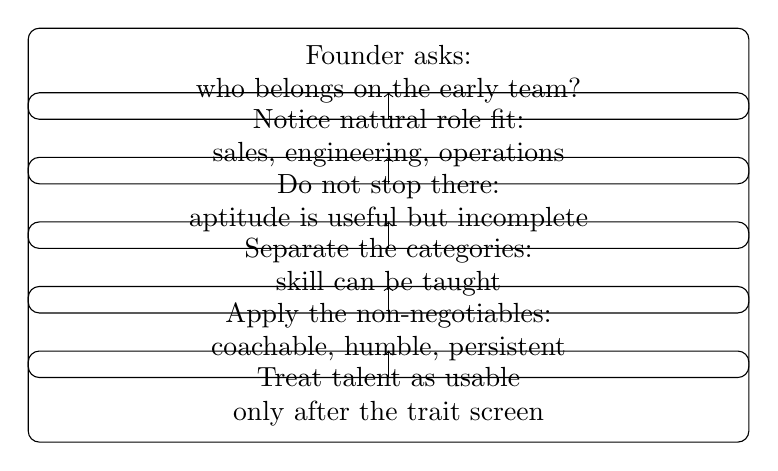
\begin{tikzpicture}[
  node distance=0.82cm,
  every node/.style={
    draw,
    rounded corners,
    align=center,
    text width=0.72\linewidth,
    inner sep=6pt
  },
  every path/.style={->}
]
\node (q) {Founder asks:\\ who belongs on the early team?};
\node (role) [below of=q] {Notice natural role fit:\\ sales, engineering, operations};
\node (limit) [below of=role] {Do not stop there:\\ aptitude is useful but incomplete};
\node (skill) [below of=limit] {Separate the categories:\\ skill can be taught};
\node (trait) [below of=skill] {Apply the non-negotiables:\\ coachable, humble, persistent};
\node (decision) [below of=trait] {Treat talent as usable\\ only after the trait screen};

\draw (q) -- (role);
\draw (role) -- (limit);
\draw (limit) -- (skill);
\draw (skill) -- (trait);
\draw (trait) -- (decision);
\end{tikzpicture}
\end{figure}

In the most compact logical form, the hiring filter is:
\begin{equation}
  \operatorname{Hire}(c)
  \Rightarrow
  \operatorname{RoleFit}(c)
  \land
  \operatorname{TraitClear}(c).
\end{equation}
The decision rule is stronger in practice:
\begin{equation}
  \operatorname{RoleFit}(c)
  \land
  \operatorname{TraitClear}(c)
  \longrightarrow
  \text{candidate worth serious consideration}.
\end{equation}
Role fit tells us where the person might help. Trait fit tells us whether the company can actually build with that person.

\section{Worked Example: The Talented Sales Rep}

The interview closes by testing the rule against an attractive candidate. Suppose \(c\) is a strong sales representative at a generic outside company, called ``XYZ company'' in the transcript. We observe:
\begin{equation}
  \operatorname{RoleType}(c)=\text{sales},
  \qquad
  \operatorname{Talent}(c)=1.
\end{equation}
That is real evidence. The speaker even grants that it is good. But it does not imply success in this company:
\begin{equation}
  \operatorname{Talent}(c)
  \lor
  \operatorname{School}(c)
  \lor
  \operatorname{Referral}(c)
  \nRightarrow
  \operatorname{SuccessHere}(c).
\end{equation}

The worked screen runs in the same order as the interview:
\begin{enumerate}
  \item Identify the visible role lane:
  \[
    \operatorname{RoleType}(c)=\text{sales}.
  \]
  \item Acknowledge the visible talent:
  \[
    \operatorname{Talent}(c)=1.
  \]
  \item Refuse to treat talent, school, or referral as decisive:
  \[
    \operatorname{PrestigeSignal}(c)
    \nRightarrow
    \operatorname{SuccessHere}(c).
  \]
  \item Apply the trait test:
  \[
    \begin{aligned}
      \operatorname{TraitClear}(c)
      &=
      \operatorname{Coachable}(c)
      \land
      \operatorname{Humble}(c) \\
      &\land
      \operatorname{Persistent}(c).
    \end{aligned}
  \]
\end{enumerate}
Only after this sequence does the talent become operationally valuable. Without the trait screen, talent remains an outside signal rather than an inside capability.

\section{Summary}

The passage gives a compact founder's rule for early team selection. First, notice what people are naturally good at: sales, engineering, operations, or another useful lane. Then refuse to confuse that visible aptitude with a complete hiring decision. The decisive distinction is between skills, which the speaker believes can be taught, and traits, which he treats as non-negotiable.

The final filter is:
\begin{equation}
  \boxed{
    \operatorname{Hire}(c)
    \text{ only after }
    \operatorname{RoleFit}(c)
    \text{ and }
    \operatorname{TraitClear}(c)
  }.
\end{equation}
For this speaker, the trait screen is coachability, humility, and persistence. Talent matters, but it matters after those conditions are met.
